\chapter{RF Fundamentals}\label{fundamentals}

\minitoc 

\clearpage
\section*{Objectives}
To develop a sound, practical understanding of:
\begin{itemize}

\item radio frequency behaviour (propagation characteristics, frequency band selection and range);

\item the variation in the relationship between power and distance for different frequencies;

\item impact of Interference (sources of noise and interference);

\item antenna systems (type selection);

\item channel bandwidth (vs frequency bands);

\item the Shannon-Hartley law
 
\item system gain; 

\item reflection and refraction of wireless signals;

\item multipath propagation and how OFDM overcomes it.

\end{itemize}


\section{Wireless Signal Characteristics}

\subsection{Power vs distance}

The power of an electromagnetic signal reduces over distance because,
as the signal propagates through space, the energy it carries is spread
over a larger area. This is illustrated in Figure \ref{inversesquarelaw}.
\begin{figure}
	\centering
	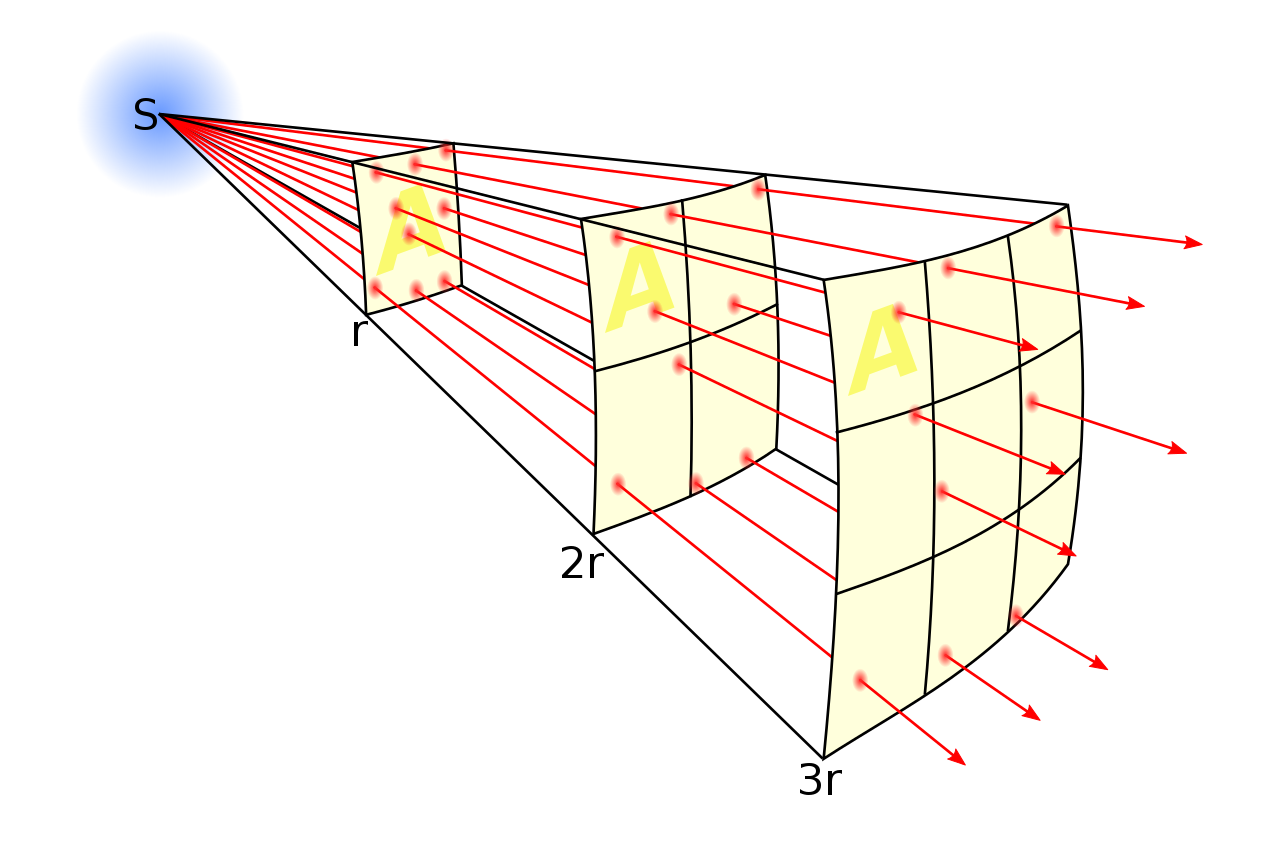
\includegraphics[width=10cm]{Inverse_square_law_svg}
	\caption{The inverse square law (By Borb, CC BY-SA 3.0, https://commons.wikimedia.org/w/index.php?curid=3816716)}
	\label{inversesquarelaw}
\end{figure}

From the principle illustrated in Figure \ref{inversesquarelaw}, we can conclude,
more precisely, that the power of a signal decreases in proportion to the square of the distance
between the sender and the receiver:
\begin{equation}
	P_d = \frac{1}{d^2} P_1,
\end{equation}
in which $P_d$ denotes the power of the signal received at distance $d$ from the transmitter.

This assumes that the signal is not absorbed by the medium; for example, if the space between
the sending antenna and the receiving antenna is completely empty -- a vacuum -- we can expect
the inverse square law to be exact. But if the space has some contents, e.g. air, glass, water, 
mist, clouds, rain, etc, then there will be some absorption of energy in the intervening space
and the inverse square law will not hold exactly.

\subsection{Power vs Frequency }

The atmosphere is not completely transparent for light. Some frequencies are absorbed
more than others. The absorption of a proportion of the light passing through
a medium, such as the atmosphere, which is not completely transparent, introduces
additional loss which is also proportional to a power of the distance between the
transmitter and the receiver. If the medium is completely transparent, the additional
gain (although it is actually a loss, we refer to it as a gain less than $1$
to simplify its numerical expression) due to the medium will be $d^0=1$, where
$d$ is the distance. If the media does introduce loss, this gain will be $d^{-a}$
for some $a>0$.

[David, here we need to introduce a figure which shows the loss, as this power of $d$,
at different frequencies, due to oxygen, etc.

This would also be a good place to introduce a discussion of the spectrum used
in Star Link, as an example of the sort of compromise which can be adopted, when
a frequency has loss, but we can work with it.
]

For best communication, we naturally prefer to use frequencies of light
which have as little loss as possible. However, because modern communication technology is
highly efficient, and there is so much commercial pressure to use the available
spectrum (frequencies) for communication, we do not simply avoid using frequencies
with higher loss, but instead we make use of the best methods of modulation, filtering
and receiver designs so that we can make use of all frequencies by adapting to their
characteristics.

\subsection{Noise and interference}

Noise is present in all communication systems. It is caused by heat, which
is present in all devices and media involved in a communication system,
and by electromagnetic radiation, which is also present everywhere. Other
communications taking place in the same, or a nearby, location will
also cause interference, although in many cases such signals can also be
treated as noise. The impact of noise on the capacity of a communication
system has been precisely quantified in \S\ref{shannonhartley}.

\section{Antenna Design and Choice}

Antenna design is tricky to explain, and to do. Fortunately,
most of us do not need to {\em design} antennas, but merely to
choose the appropriate one from a small range of alternatives, in
a certain situation. Nevertheless, there some simple principles
which we can easily learn that make it a lot easier to make these
choices correctly.

\subsection{Dipole Antennas}

A short dipole antenna is depicted in Figure \ref{dipole}.
\begin{figure}
	\centering
	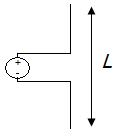
\includegraphics[width=6cm]{dipole}
	\caption{A short dipole antenna (from \url{https://www.antenna-theory.com/antennas/shortdipole.php})}
	\label{dipole}
\end{figure}
When stimalated by an oscillating voltage at its centre, this antenna causes propagation of an electromagnetic
signal. This is because, due to the physical law described by Maxwell's equations, 
the {\em current} in the arms of the antenna directly cause a time-varyig magnetic field
in the vicinity of these arms, which then, because it varies in time and space, also leads
to a time-varying electrical field. Both these fields then propagate away from the antenna.
These propagating fields constitute elemctromagnetic radiation, i.e. radio waves. If this field
is, moreover, varied in time according to a {\em message}, this details of this message will
be detectable at a receiver some distance away.

The strength of this signal is, naturally enough, proportional to the strength of the electrical signal
at the source, and also to the length of the arms, so long as the antenna is {\em short}.
An antenna is regarded as short only if it is shorter, in length, than a quarter of a wavelength,
for the particular frequency of the original signal. As the antenna approaches a half wavelength, in
size, the law of signal strength increasing with length of the antenna breaks down, and once
the antenna is {\em longer} than half a wavelength, transmitted signal strength starts reducing.

Simple dipole antennas must, therefore, be of length in roughly the range 1/4 to 1/2 the wavelength
of the signal. 


\subsection{Frequency dependence}

The idea that the physical dimensions, and shape, of an antenna depends critically on the
frequencies being transmitted, or received, is not only true for dipole antennas. If an antenna
is designed for frequency $f$, but used for frequency $2f$, its performance will seriously
oompromised.

\subsection{Reciprocity}

Reciprocity is the principle that transmission and reception of electromagnetic signals
from an electrically stimulated (or monitored) antenna obey ``exactly'' the same physical
principles. Here is one statement of this principle, from \cite{antennatheory}:
\begin{quote}\em
Reciprocity is one of the most useful (and fortunate) property of
antennas. Reciprocity states that the receive and transmit properties of
an antenna are identical. Hence, antennas do not have distinct transmit
and receive radiation patterns - if you know the radiation pattern in the
transmit mode then you also know the pattern in the receive mode. This
makes things much simpler, as you can imagine.  
\end{quote}

Although it is not completely obvious how to apply this principle, the important
takehome message is that our understanding of transmission, such as it is,
can be used to help our understanding of reception of signals, and conversely.
This is helpful. In particular, an antenna which is well designed for transmission,
in a particular context (for example, for a certain frequency range, will also be well designed for receiving signals, in the
same context.

\subsection{Multiple Input Multiple Output (MIMO)}\label{mimo}

If a larger antenna than 1/4-1/2 wavelength is desired, while retaining the simplicity of the
dipole structure, rather than making the dipole itself longer, it is necessary to use multiple
antennas, each of which has the preferred 1/4-1/2 wavelength length. If the signals from these
multiple antennas have to be combined by carefully selected coefficients, determined by measurements
of the channel frequency response, the effective signal to noise ratio can be steadily improved
as more antennas are added. 

This is particularly important for signals with short wavelengths, because no single
antenna will be able to receive a strong signal by itself. Thus, for higher frequencies,
it is likely to be essential to use multiple antennas for both sending and receiving signals.

\section{The Shannon-Hartley law}\label{shannonhartley}

Supposing a communication channel is not noise free, but has noise with power level $N$, the
error rate of the received signal will be non-zero. The formula of Hartley and
Shannon\index{Shannon} takes this into account, and gives the maximum data rate in the presence of noise,
as:
$$
C \leq B \log_{2} (1 + S/N). 
$$
where $C$ is the channel capacity, in bits/s, $B$ is the bandwidth, in Hz, and $S/N$ is the 
signal-to-noise ratio (SNR)\index{signal-to-noise ratio (SNR},
which is the ratio of the power levels of the signal and the noise, 
at the receiver. 

\begin{sbexample}{The Shannon capacity of a channel}%
As an example consider we have a radio channel with bandwidth 10
\textsc{MH}z. Say the received signal level is 2 m\textsc{W}, and the
noise level is 0.04 m\textsc{W}. What is the Shannon Capacity of the
channel?  
$$ 
\hbox{SNR} = S/N = 2mW / 0.04 mW = 50 .  
$$

$$
C = 10\times 10^{6} \times \log_{2}(1 + \hbox{SNR}) = 10^{7} \times 5.67 = 56.7 \hbox{Mbit/sec} .
$$
\end{sbexample}


Note that this capacity value is higher than the Nyquist bandwidth of
the channel. To achieve this high value of capacity it is necessary to
use more than 2 voltage levels to represent bits ($M > 2$), this was
rarely done in practice in the past, however, with the introduction of
OFDM it has become more common to use modulation techniques like QPSK
(Quadrature Phase Shift Keying)\index{Quadrature Phase Shift Keying
(QPSK)} in which more than two symbols are transmitted per time slot,
and hence it becomes possible to exceed the Nyquist rate.

The Shannon Capacity formula also provides a general idea of how much noise we can 
tolerate on a channel. Suppose we have a radio bandwidth of 30 MHz, as for example in the
802.11b channel, and we want to transmit data at 11 Mbit/sec. Then,
\begin{eqnarray}\nonumber
\hbox{SNR} &=& 2(C/B)-1 \\
\nonumber
\hbox{SNR} &=& 2(11*10^{6}/30*10^{6})-1 \\
\nonumber
\hbox{SNR} &=& 1.28-1=0.28
\end{eqnarray}

This corresponds to a signal \textit{loss} of 5.38 dB, which indicates
that the signal power can actually be \textit{less than} the channel
noise level.

\begin{exercise}{Using Shannon's capacity formula}
Consider we have a channel with bandwidth 125 MHz. Suppose the received
signal level is 5 mW, and the noise level is 1.2 mW. What is the Shannon capacity of
the channel?
\end{exercise}


\section{System Gain}

\subsection{Free space loss}

\subsection{Antenna gain}

\subsection{Feeder loss}

\subsection{Transmitter power}

\subsection{Receiver sensitivity}


\section{Reflection and Refraction}

\subsection{Multipath Propagation}
\begin{figure}
	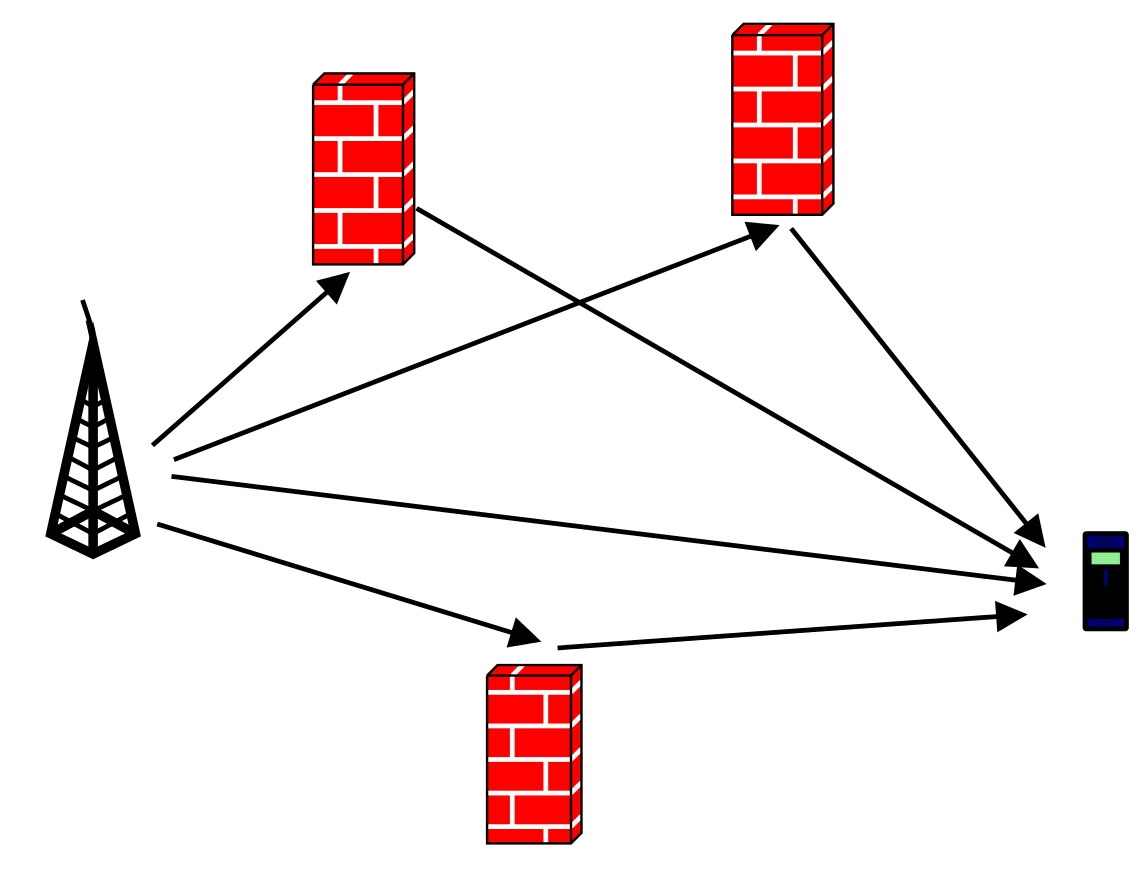
\includegraphics[width=10cm]{multipathproblem.png}
	\caption{Multipath propagation}\label{multipath}
\end{figure}
Wireless signals pass along multiple paths of different gain, and delay
as shown in Figure \ref{multipath}.
Each path can have a complex gain which depends on the types of
reflections or refraction which occur along the path. Nevertheless, each
frequency does, in general, have a well-defined complex gain, which
can be estimated.

This is the multipath problem.

\subsection{Orthogonal Frequency Division Multiplexing}
OFDM solves the multipath problem. In brief, it works as
follows:
\begin{itemize}
\item Divide spectrum up into bands
\item Relative to a frame, bands are {\em orthogonal}
\item Estimate the complex gain of each frequency
\item This overcomes multipath interference
\item Transmit over all frequencies at once
\item Each frame must include a cyclic continuation
\end{itemize}

The OFDM concept was first discovered many decades ago, but
was fully proved, with an implementation, first, by Australia's CSIRO.
They were awarded a patent on the concept, which was adopted in 802.11 
from 802.11a. 802.11b was the last non-OFDM wifi.
